\section{Transformer}

\subsection{Output}
\begin{frame}[c]{Output}
    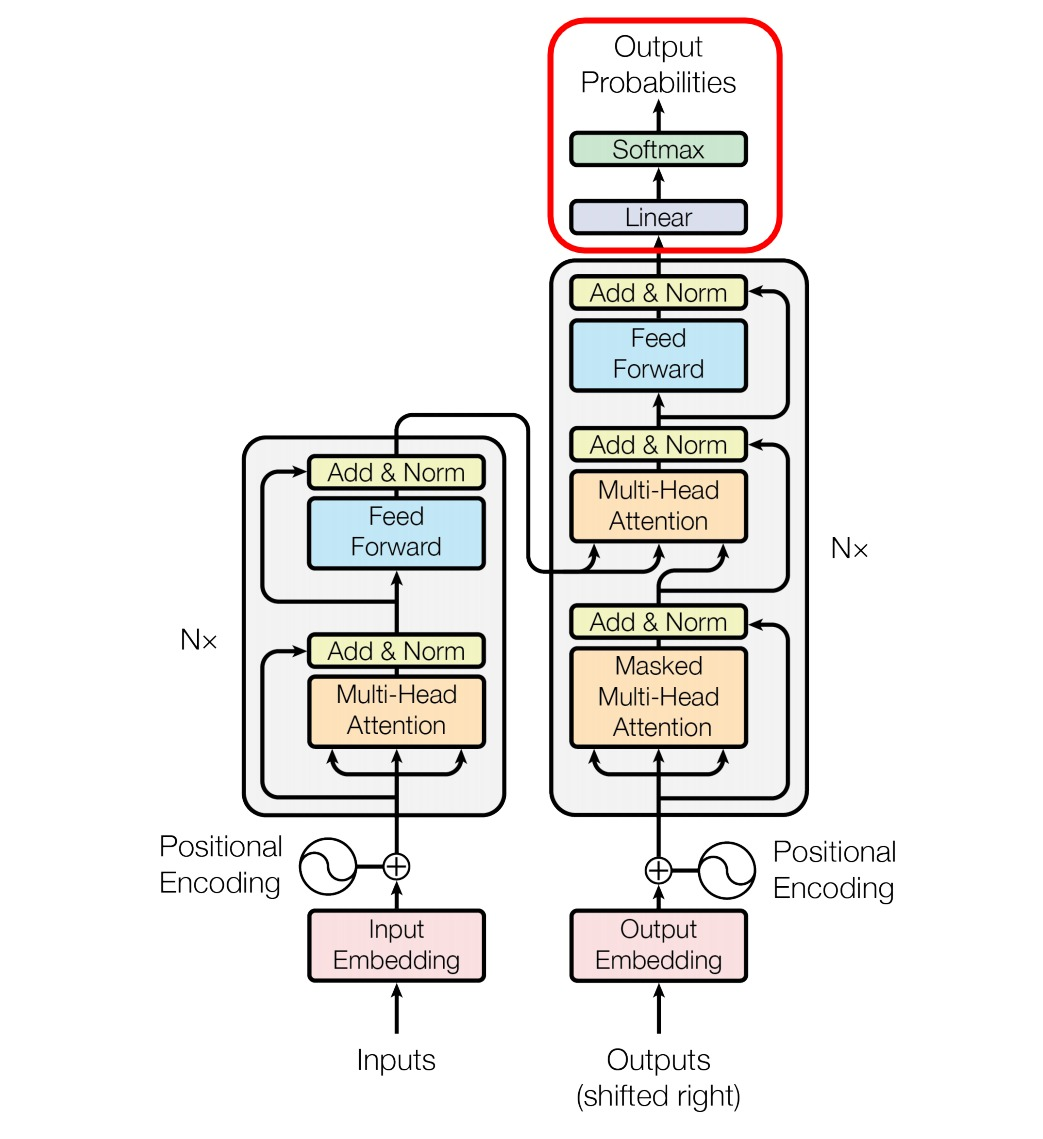
\includegraphics[height=0.9\textheight,clip,trim=120 0 120 0]{transformer_output}
    \raisebox{3em}{\gray{Image Adapted from \cite{vaswani_attention_2017}}}
    \pnote{
        followed by topk selection
    }
\end{frame}

\begin{frame}[c]{Parameters}
    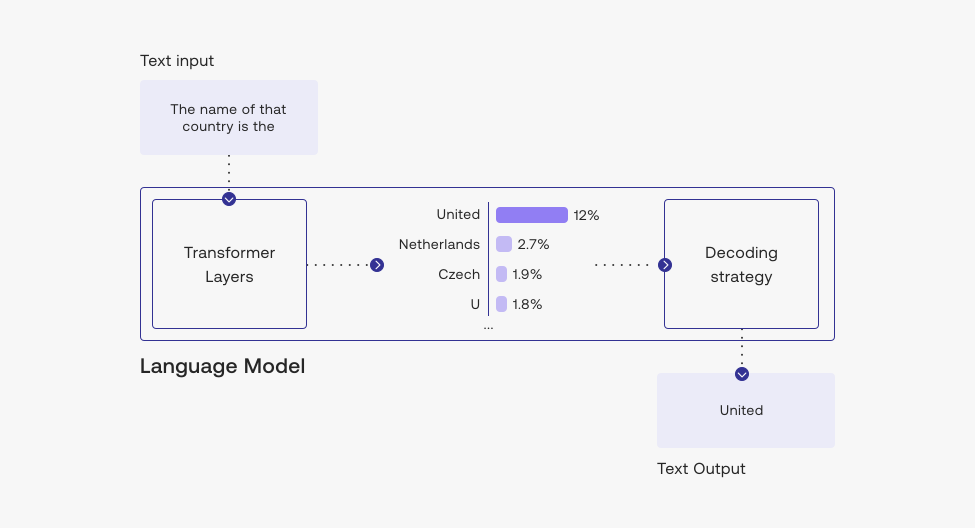
\includegraphics[width=\textwidth]{decoding_strategy} \\
    \gray{Image Source: \cite{cohereaidocs_topk_2022}}
\end{frame}


\begin{frame}[c]{Temperature, Top-k and Top-p}
    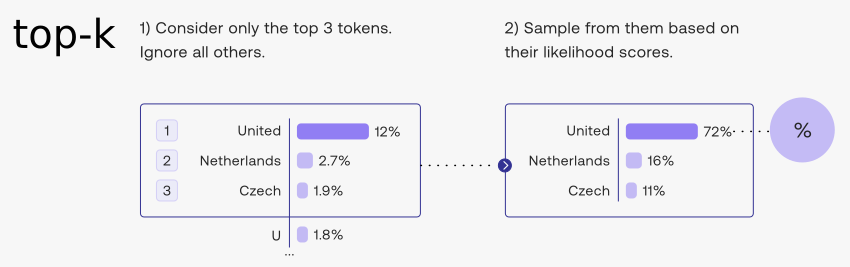
\includegraphics[width=\textwidth]{decoding_topk} \\
    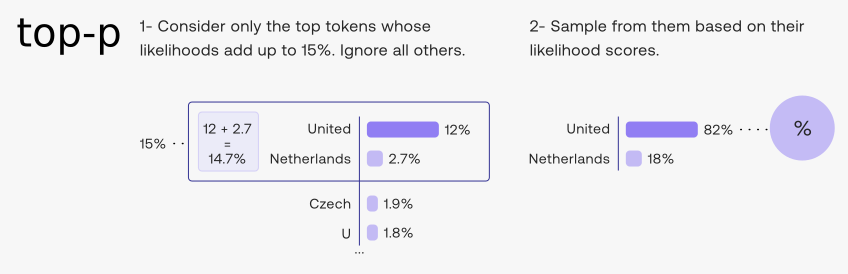
\includegraphics[width=\textwidth]{decoding_topp} \\
    \gray{Image Source: \cite{cohereaidocs_topk_2022}}
    \pnote{
        Temperature is non-linear rescaling of values, increasing chance of
        lower-likelihood predictions to be chosen.
    }
\end{frame}

\subsection{Dimensions}
\begin{frame}[c]{Dimensions at Each Step}
    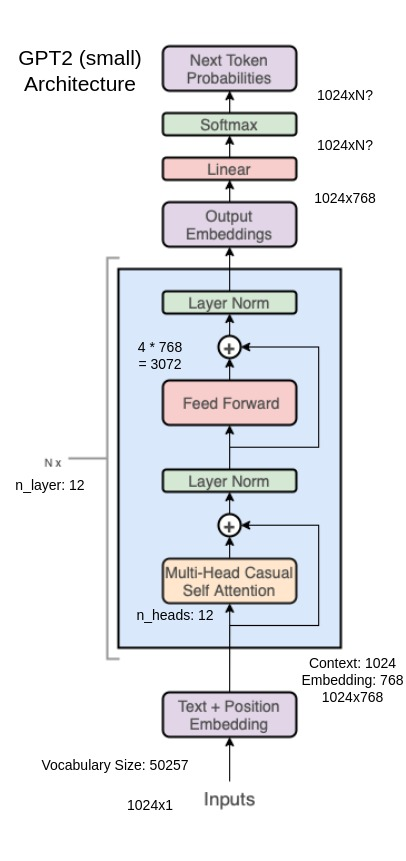
\includegraphics[height=0.9\textheight]{gpt2_decoder_dims}
    \raisebox{3em}{\gray{Image Adapted from: \cite{mody_gpt_2023}}}
    \pnote{
        Dimensions represent my current understanding
    }
\end{frame}

\begin{frame}[c]{Dimensions II}
    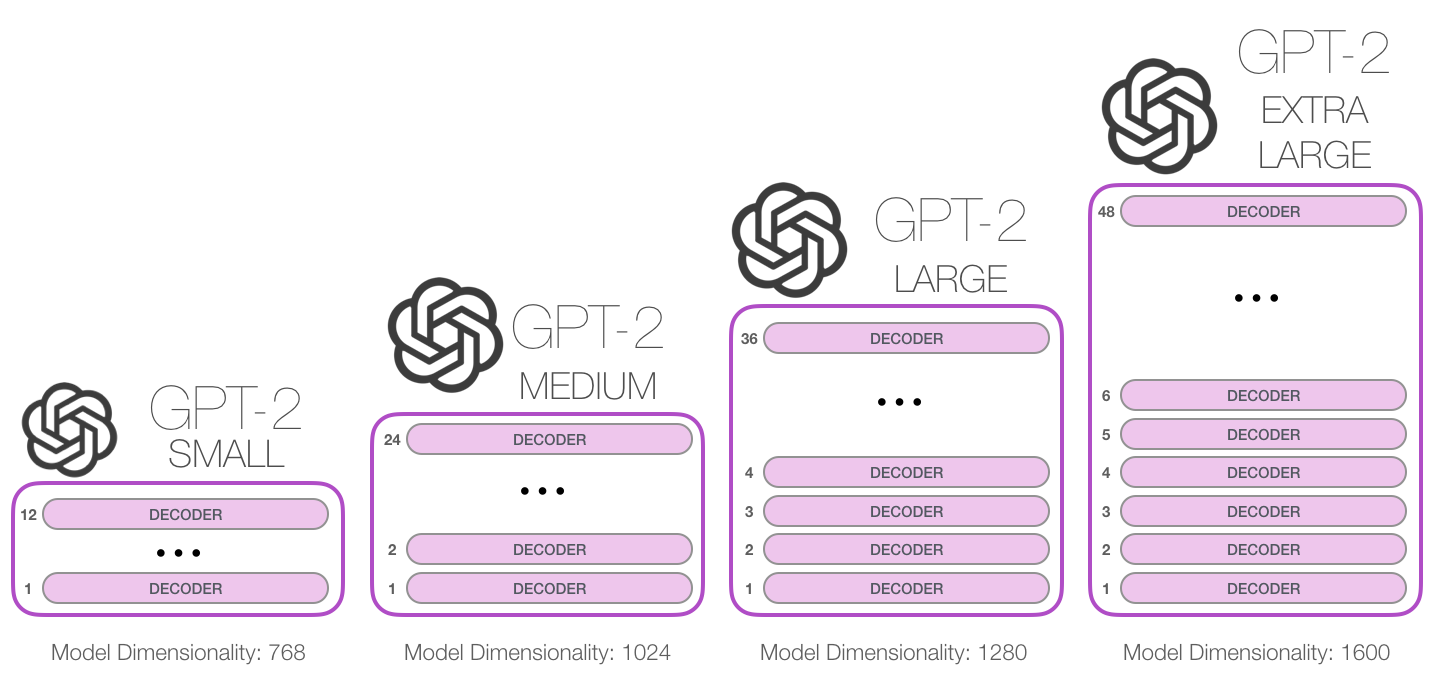
\includegraphics[width=\textwidth]{gpt2-sizes} \\
    \gray{Image Source: \cite{alammar_illustrated_2019}}
\end{frame}


\subsection{Putting it all Together}
\begin{frame}[c]{Full Architecture}
    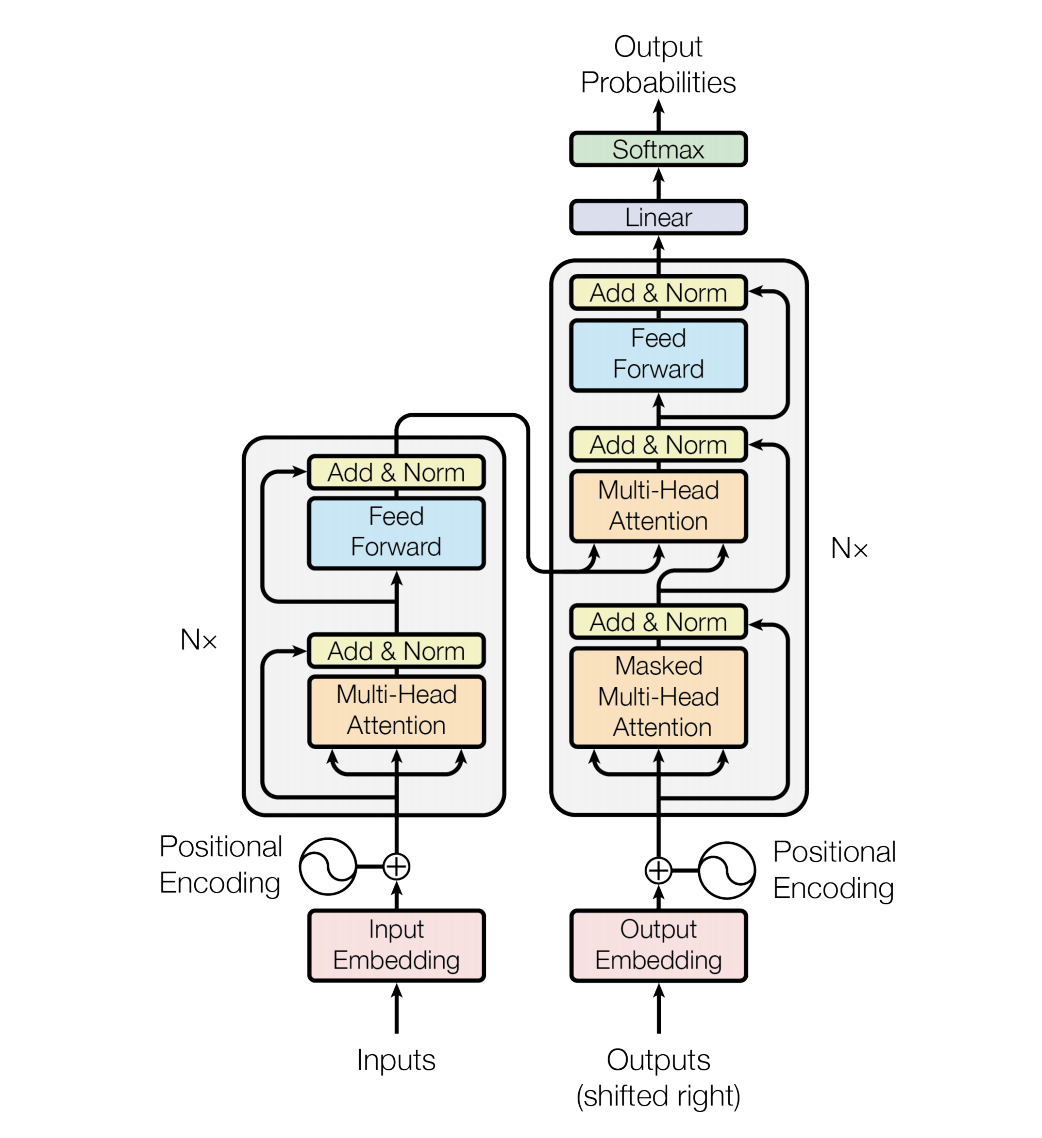
\includegraphics[height=0.9\textheight]{transformer}
    \raisebox{3em}{\gray{Image Source: \cite{vaswani_attention_2017}}}
\end{frame}

\subsection{Interpretation}
\begin{frame}[c]{One Prevalent Interpretation: Solving ODEs}
    \large
    \begin{aquote}{Lu et al., 2019 \cite{lu_understanding_2019}}
        {\em ... the Transformer can be mathematically interpreted as
        a} numerical Ordinary Differential Equation (ODE) solver for a
        convection-diffusion equation in a multi-particle dynamic
        system.
    \end{aquote}
\end{frame}


\begin{frame}[c]{A Better ODE Solver}
    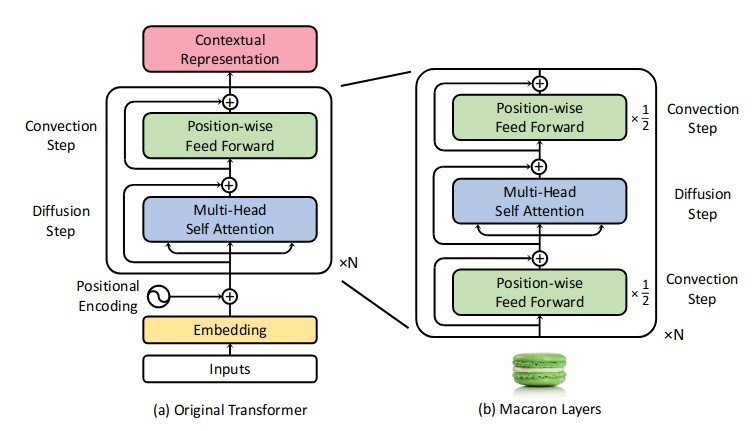
\includegraphics[width=\textwidth]{macaron_layers} \\
    \large
    For solving, use a Strang-Marchuk Splitting scheme instead of Lie-Trotter \\
    \normalsize
    \gray{Image Source: \cite{lu_understanding_2019}}
    (For details on solving methods see \cite{geiser_decomposition_2009})
    % TODO: move image source text above the additional text.
    % Doing so currently results in text overflowing of the slide, due to
    % additional space in the newline like that, for some weird reason.
    \pnote{
        they clearly showed that it could be interpreted as physical system
        with particles (tokens) interacting. For that, the solver could be
        improved. \\
        However, while they did improve results, they only did so marginally.
        I assume they didn't use it fully, more experiments necessary.
    }
\end{frame}

\begin{frame}[c]{As High-Order Nonlinearity}
    \large
    \begin{aquote}{Ye et al. 2023, Towards ... \cite{ye_understanding_2023}}
        However, we find only a weak consistency exists between the attention
        weights of features and their importance. We verify the feature map
        multiplication that brings about \textbf{high-order non-linearity into CNNs is
        crucial for the effectiveness} of attention mechanism.
    \end{aquote}
\end{frame}


\begin{frame}[c]{In-Context Optimization}
    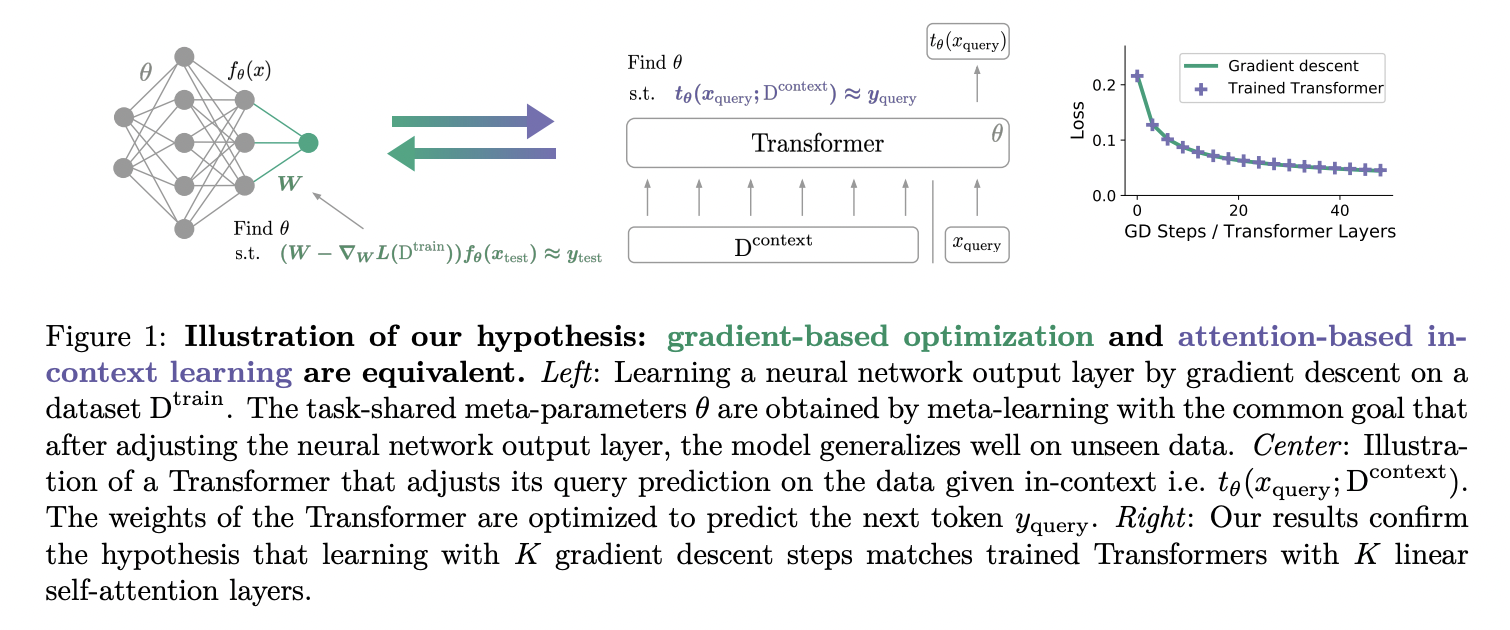
\includegraphics[width=\textwidth]{in-context} \\
    \gray{Image Source: \cite{vonoswald_transformers_2022}}
        \begin{aquote}{Transformers Learn In-Context \cite{vonoswald_transformers_2022}}
            ... training Transformers ... can be closely related to well-known
            gradient-based meta-learning formulations.
        \end{aquote}
    \pnote{
        Not sure if not actually a product of mesa-optimization \\
        \\
        information hazard note on mesa optimizers
    }
\end{frame}

\subsection{Architecture Improvements}
\begin{frame}[c]{Sparse Transformer: $O(n \sqrt{n})$ instead of $O(n^2)$}
    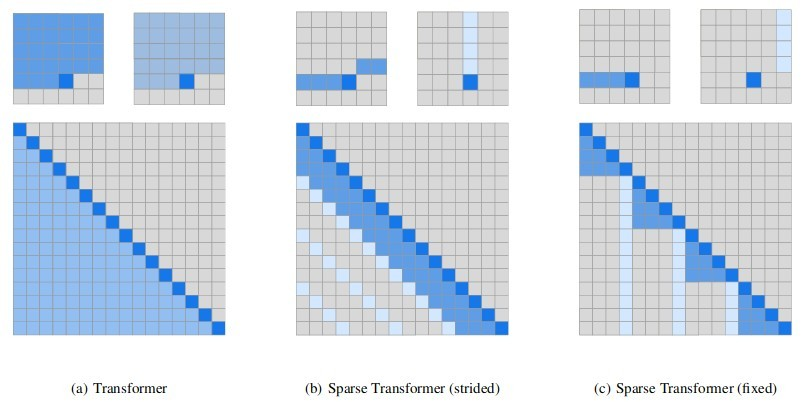
\includegraphics[width=\textwidth]{sparse_transformer} \\
    \normalsize
    \gray{Image Source: \cite{child_generating_2019}} \\
    \large
    Used first in the GPT3 family of models. \\
    A lot of other patterns are possible too
    \pnote{
    Even the original GPT didn't use 'full' transformers, but Sparse Transformer \\
    Runtime: O(n sqrt n) instead of O( n * n ) \\
    \\
    Obviously a huge benefit if you can get substantially reduced runtime \\
    for the same performance
}
\end{frame}


\begin{frame}[c]{FlashAttention}
    \large
    They realized that the bottleneck wasn't compute, but IO. \\
    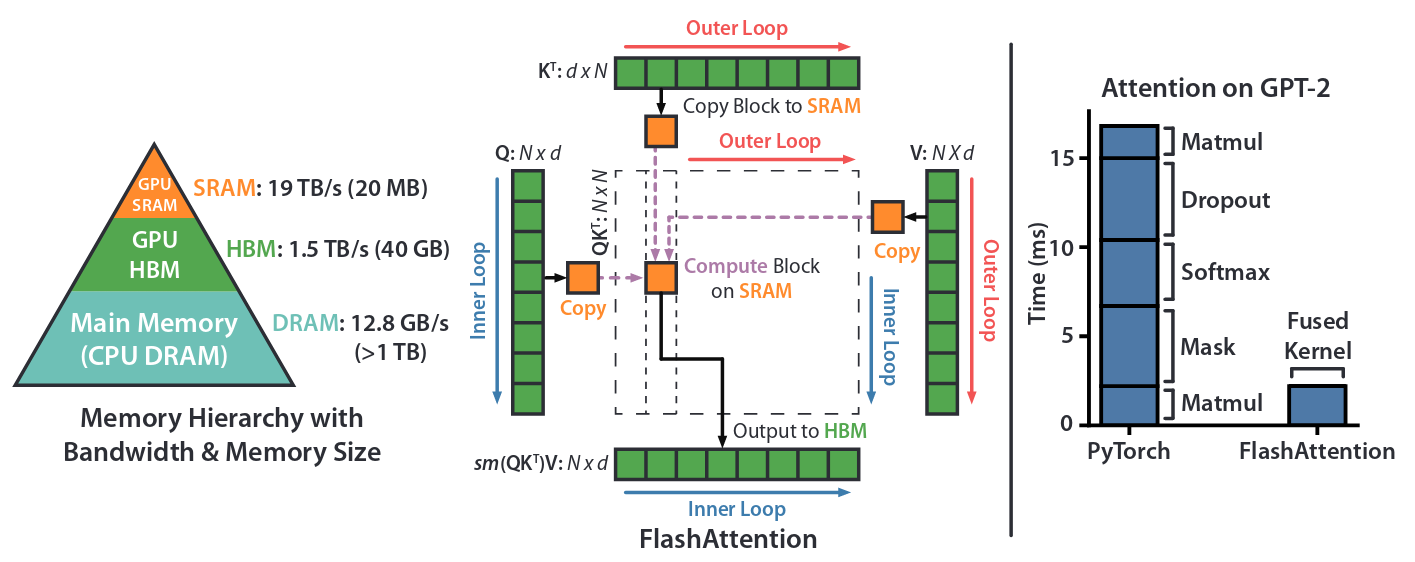
\includegraphics[width=\textwidth]{flashattention_memory} \\
    \gray{Image Source: \cite{dao_flashattention_2022}} \\
    \large
    Used first in the GPT4 family of models
    \pnote{
        From what we know, GPT4 is using a variant of FlashAttention
    }
\end{frame}


\begin{frame}[c]{FlashAttention Benchmarks}
    \large
    \begin{tabular}{c|ccc}
        Attention & Standard & FlashAttention & Ratio \\ \hline
        GFLOPs & 66.6  & 75.2 & 0.89 \\
        HBM R/W & 40.3 & 4.4 & 9.16 \\
        Runtime (ms) & 41.7 & 7.3 & 5.71 \\
    \end{tabular} \newline \newline
    \normalsize
    \gray{Table from \cite{dao_flashattention_2022}} \\
    \large
    Note that Standard Attention is $O(n^2)$ in compute.
\end{frame}

\subsection{Modern Transformer Architecture}

\begin{frame}[c]{Transformer with commonly used improvements}
    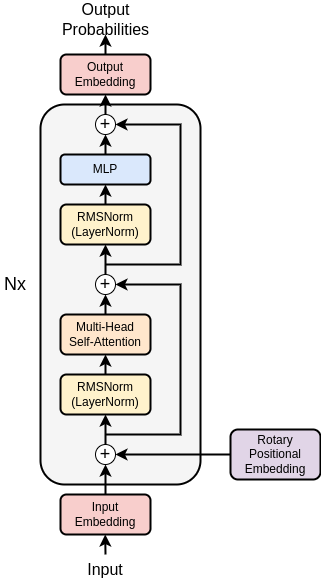
\includegraphics[height=0.9\textheight]{modern_transformer}
    \raisebox{3em}{\gray{Image Source: Self-Creation}}
\end{frame}

